%%%%%%%%%%%%%%%%%%%%%%%%%%%%%%%%%%%%%%%%%%%%%%%%%%%%%%%%%%%%%%%%%%%%%%%%%%%%%%%%
% Template for USENIX papers.
%
% History:
%
% - TEMPLATE for Usenix papers, specifically to meet requirements of
%   USENIX '05. originally a template for producing IEEE-format
%   articles using LaTeX. written by Matthew Ward, CS Department,
%   Worcester Polytechnic Institute. adapted by David Beazley for his
%   excellent SWIG paper in Proceedings, Tcl 96. turned into a
%   smartass generic template by De Clarke, with thanks to both the
%   above pioneers. Use at your own risk. Complaints to /dev/null.
%   Make it two column with no page numbering, default is 10 point.
%
% - Munged by Fred Douglis <douglis@research.att.com> 10/97 to
%   separate the .sty file from the LaTeX source template, so that
%   people can more easily include the .sty file into an existing
%   document. Also changed to more closely follow the style guidelines
%   as represented by the Word sample file.
%
% - Note that since 2010, USENIX does not require endnotes. If you
%   want foot of page notes, don't include the endnotes package in the
%   usepackage command, below.
% - This version uses the latex2e styles, not the very ancient 2.09
%   stuff.
%
% - Updated July 2018: Text block size changed from 6.5" to 7"
%
% - Updated Dec 2018 for ATC'19:
%
%   * Revised text to pass HotCRP's auto-formatting check, with
%     hotcrp.settings.submission_form.body_font_size=10pt, and
%     hotcrp.settings.submission_form.line_height=12pt
%
%   * Switched from \endnote-s to \footnote-s to match Usenix's policy.
%
%   * \section* => \begin{abstract} ... \end{abstract}
%
%   * Make template self-contained in terms of bibtex entires, to allow
%     this file to be compiled. (And changing refs style to 'plain'.)
%
%   * Make template self-contained in terms of figures, to
%     allow this file to be compiled. 
%
%   * Added packages for hyperref, embedding fonts, and improving
%     appearance.
%   
%   * Removed outdated text.
%
%%%%%%%%%%%%%%%%%%%%%%%%%%%%%%%%%%%%%%%%%%%%%%%%%%%%%%%%%%%%%%%%%%%%%%%%%%%%%%%%

\documentclass[letterpaper,twocolumn,10pt]{article}
\usepackage{usenix-2020-09}

% to be able to draw some self-contained figs
\usepackage{tikz}
\usepackage{amsmath}
\usepackage{float}
\usepackage{enumitem}


%-------------------------------------------------------------------------------
\begin{document}
%-------------------------------------------------------------------------------

%don't want date printed
\date{}

% make title bold and 14 pt font (Latex default is non-bold, 16 pt)
\title{\Large Investigation on
    HyperEnclave: An Open and Cross-platform Trusted Execution Environment}

%for single author (just remove % characters)
\author{
{\rm Ahmet Turkmen}\\
Technical University of Munich
\and
{\rm Mert Sarac}\\
Technical University of Munich
% copy the following lines to add more authors
% \and
% {\rm Name}\\
%Name Institution
} % end author

\maketitle


%-------------------------------------------------------------------------------
\begin{abstract}
%-------------------------------------------------------------------------------
Trusted executed environments (TEEs) are isolated, secure environments designed to protect sensitive or confidential data. They prevent unauthorized access and detect infiltration attempts and react to them. Enclaves do have significant drawbacks such as the difficulties in auditing brought on by closed-source technology and fixed-mode operation. The usage of "HyperEnclave," which is open source, cross-platform, and provides a variety of flexible running modes, is suggested as a solution for these constraints. It may also be immune to some types of attacks that existing TEEs are unable to withstand. This paper aims to evaluate HyperEnclave technology in terms of what it promises, which problems it covers, how to solve them, and its design.
\end{abstract}


%-------------------------------------------------------------------------------
\section{Introduction and Problem Definition}
%-------------------------------------------------------------------------------

An enclave is a secure and isolated environment within a larger network or infrastructure that is designed to protect sensitive or classified information. \cite{whitepaper} These enclaves prevent unauthorized access to the information stored within them and detect and respond to any attempts at intrusion. They are isolated from larger networks or infrastructure through dedicated hardware or software, or by physically separating the enclave from the rest of the network. Beyond traditional security measures, enclave technology offers additional levels of protection such as firewalls and encryption. Despite their high level of security, this technology also has some drawbacks. Existing trusted execution environments (TEEs) are bound to specific vendors such as Intel, AMD, ARM, and IBM. This limit enclaves to adapt to diverse workloads. Also, they are closed source which excludes the research community to audit them. In addition, current TEEs lack supporting commodity hardware without hardware or firmware changes. Another drawback is that most TEE design enforces enclaves run in a fixed mode which causes significant performance degradation for running I/O-intensive and memory-demanding tasks Finally, they are not invulnerable to all attacks even if they provide a high level of security. 

\noindent
Opposed that, a solution named “HyperEnclave” is proposed which is an open source, cross-platform TEE with multiple flexible running modes. It offers invulnerability to some specific attacks such as memory mapping attacks that current TEEs cannot handle. 

\noindent
In this paper, a detailed overview and analysis about Hyper Enclave will be mentioned.


%-------------------------------------------------------------------------------
\section{Background Information}
%-------------------------------------------------------------------------------
A trusted execution environment (TEE) is a processing environment that is isolated, secure, and integrity protected that includes processing, memory, and storage capabilities.
\cite{sabt:hal-01246364}
Being isolated makes TEEs invulnerable for most malicious actors to access and tamper with sensitive data. \cite{10.1145/2508859.2516758}

%-------------------------------------------------------------------------------

%----------------------------------------------------------------------------
\section {Importance and Challenges}
%-----------------------------------
Due to increasing privacy and security concerns TEEs are becoming crucial since sensitive information is being stored and processed through devices. However, the adaptation of TEEs on diverse workloads is not trivial and requires high engineering effort. Moreover, current TEEs are subject to exploit page attacks. The challenges can be summarized in points as follows: 
\begin{itemize}
    \item The need for minimal code base in the TCB
    \item The need to build TEEs that can run on commodity hardware without hardware or firmware changes.
    \item The need for non-trivial engineering effort to adapt HyperEnclave to other platforms such as ARM and RISC-V due to differences in instruction set architectures (ISAs).
    \item The need to minimize the attack surfaces under different enclave operation modes.
\end{itemize}

The research gap in this work is that HyperEnclave requires the virtualization extension (specifically, two-level address translation) for isolation and TPM for the root of trust and randomness. While it has been adapted to run on AMD hardware, there is no information on how it can be adapted to run on other platforms such as ARM and RISC-V. Furthermore, porting HyperEnclave to the other platforms requires non-trivial engineering effort due to a variety of instruction set architectures. In the paper, the authors state that they leave the further exploration of adapting HyperEnclave to other platforms for future work. 


%----------------------------------------------------------------------------
\section{System Overview}
%----------------------------------------------------------------------------
HyperEnclave has three main design goals which are; minimum hardware requirements, easy-to-develop, and flexible enclave modes. Minimum hardware requirements goal provided through hardware virtualization and by using the Trusted Platform Module (TPM) to provide a root of trust for the system. Easy to develop, HyperEnclave is SGX compatible, which means that porting existing SGX programs does not lead to overhead.
\newline
Overall overview of HyperEnclave can be seen in Figure 1. 
\begin{figure}[H]
    \centerline{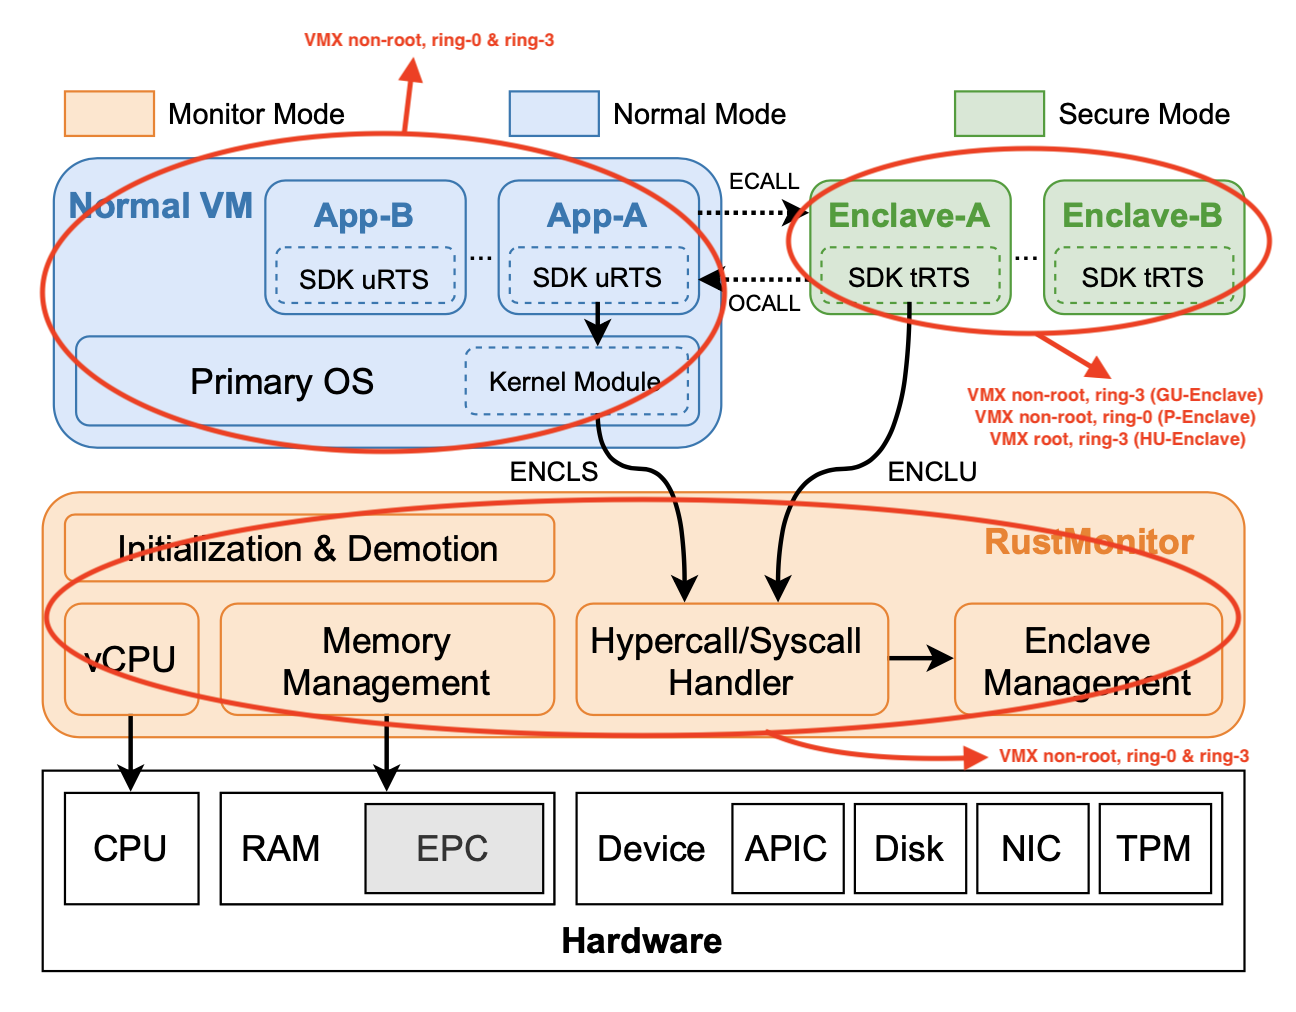
\includegraphics[scale=.42]{figures/system_overview.png}}
    \caption{System Overview}
    \label{fig}
\end{figure}

\noindent
HyperEnclave is a Trusted Execution Environment (TEE) that allows for the creation of flexible enclaves on commodity hardware without requiring any hardware or firmware changes. HyperEnclave uses hardware virtualization features such as two-level address translation and TPM for the root of trust and randomness.
Multiple modes of operation are supported as seen in given Figure 1, including the monitor mode, normal mode, and secure mode. The secure mode has different capabilities to run in a variety of VMx permissions, at ring 3 (GU Enclave) and at ring 0 (P Enclave) it can run in non-root mode in addition, at ring 3 (HU Enclave) runs in root mode. The normal mode only supports non-root modes which are at ring 0 and ring 3 as illustrated in the Figure. Similarly, Rustmonitor runs in VMX non-root mode at ring 0 and ring 3. 

\noindent
It consists of several components, including the RustMonitor, a lightweight hypervisor that manages the enclave memory and controls the enclave state transitions. The primary OS (such as Linux) and untrusted parts of applications run in normal mode.  A kernel module in the primary OS for loading and launching RustMonitor. HyperEnclave SDK is compatible with  Intel SGX SDK hence allowing for easy development and most SGX programs can run on HyperEnclave with minimal changes to the source code. HyperEnclave is prototyped on AMD servers.
HyperEnclave modes can be summarized in Figure 2.

\begin{figure}[H]
    \centerline{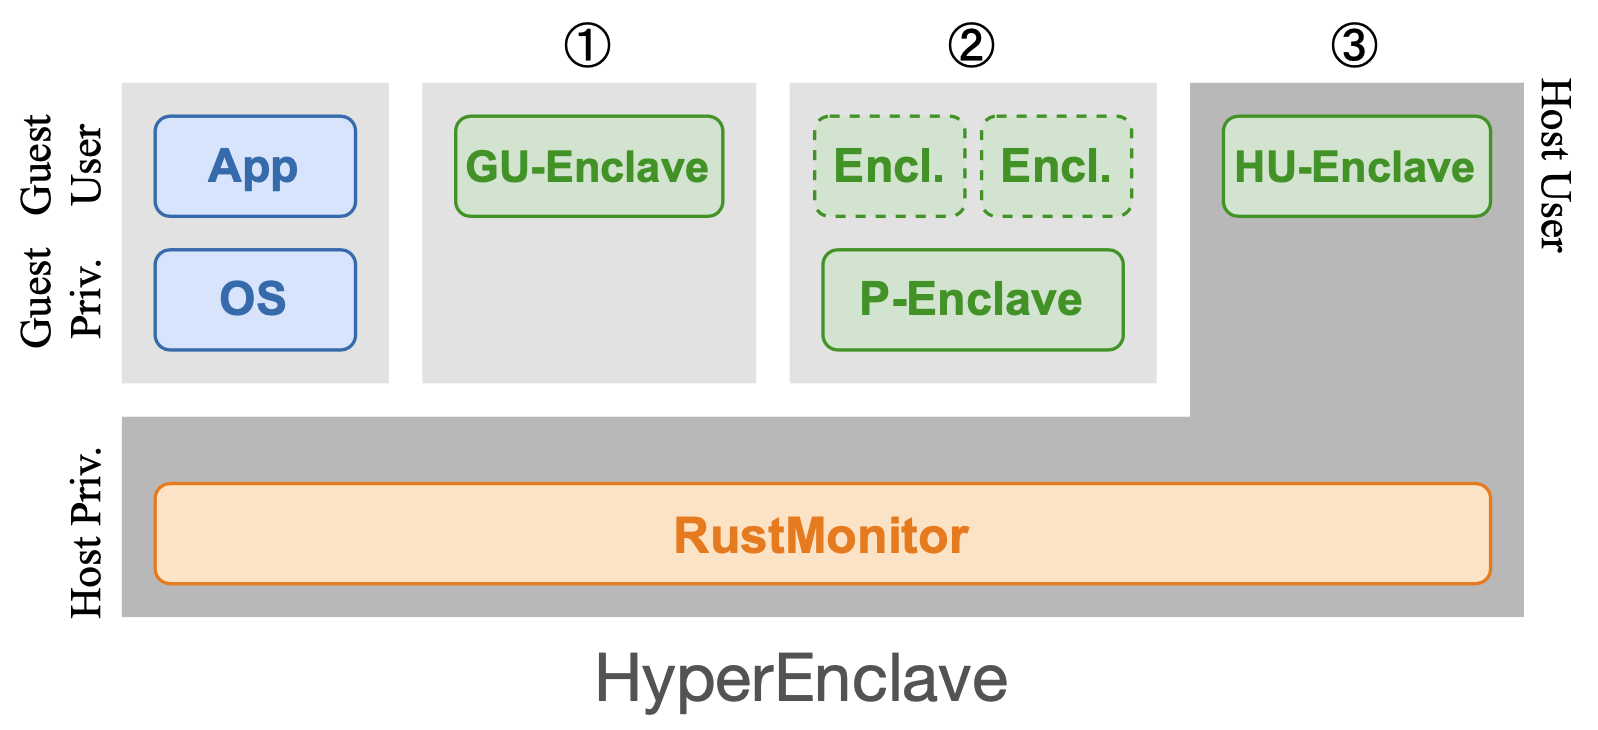
\includegraphics[scale=.15]{figures/hyperenclave_modes.png}}
    \caption{HyperEnclave modes}
    \label{fig}
\end{figure}


\begin{enumerate}[topsep=0pt, partopsep=0pt]
    \setlength\itemsep{-0.4em}
    \item GU-Enclave - basic enclave operation mode, it is used for computing intensive workloads and running in guest user mode. 
    \item P-Enclave -  privileged enclaves are running in privileged guest user mode, have access to IDT, page tables and level 1 page tables. Garbage collectors (essential in Java)  are using P-Enclave privileges. 
    \item HU-Enclave  -  running in host user mode,  provides fast world switches (according to experiments in the paper ) \textbf{hypercalls}: ∼ 880 CPU and \textbf{syscalls}: ∼ 120 CPU cycles. HU-Enclave is preferred for I/O intensive workloads
\end{enumerate}

%----------------------------------------------------------------------------



%----------------------------------------------------------------------------
\section{Evaluation}
%----------------------------------------------------------------------------
HyperEnclave is evaluated on several applications namely a lightweight web server Lighttpd and Redis which are CPU-Intensive and memory-intensive tasks in order. The evaluations were conducted by porting the OS Occlum library to the enclave SDK and measuring the performance on both HyperEnclave and Intel SGX. The experiments show that HyperEnclave has a lower overhead than SGX, and performs better on memory-intensive tasks as shown in Figure 3.

\begin{figure}[H]
    \centerline{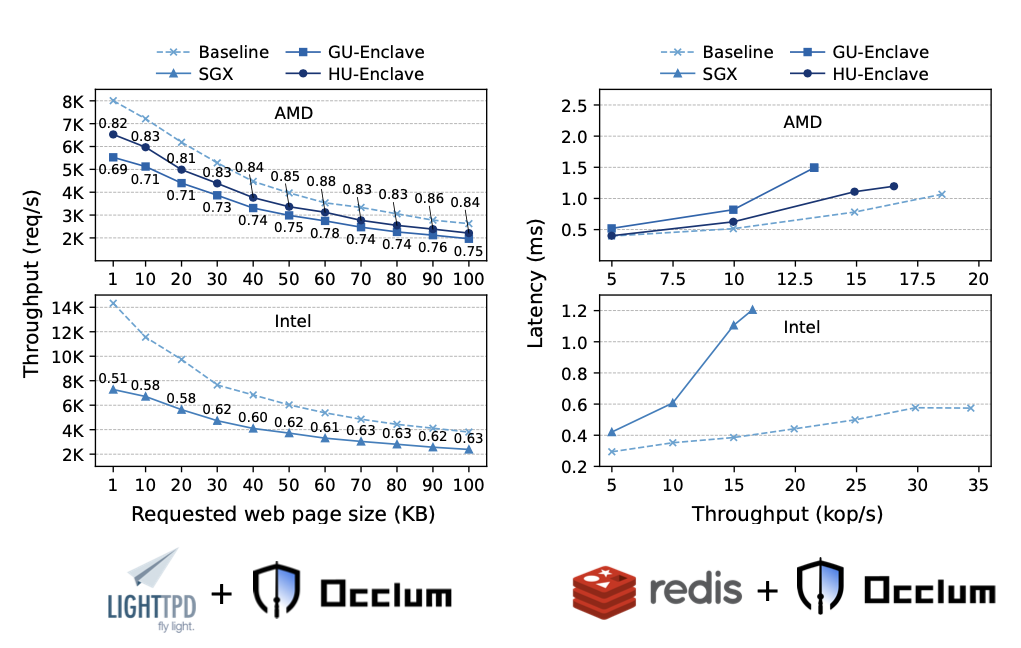
\includegraphics[scale=.29]{figures/evaluation.png}}
    \caption{Evaluation results on lighttpd+occlum and redis+occlum}
    \label{fig}
\end{figure}

\noindent
 Additionally, the performance of HyperEnclave in HU-Enclave mode is better than that of SGX in most cases. Overall, the results suggest that HyperEnclave is a promising technology for secure data processing.

\noindent
The authors provide extensive results and plots on the project repository page\footnote{https://github.com/HyperEnclave/atc22-ae}



%----------------------------------------------------------------------------
\section{Analysis of Current Work}
%-------------------------------------------------------------------------------

Throughout the research, it is shown that there have been some technical and non-technical challenges. 
The main technical challenges regarding research and need for the improvements points can be summarized as follows:

\begin{enumerate}
    \item \textbf{Enclave isolation problem}

    In current TEEs, enclaves run in a fixed mode which is very similar to HyperEnclave’s user mode so handling enclaves page tables become an issue. For example, it might cause an attack from an untrusted OS and can control its page tables which is called a memory mapping attack. To inhibit this issue, a mechanism that any updates on page tables must be verified by the hypervisor is designed. However, on x86, this mechanism leads to significant overhead, and due to still being processed by the OS, page-table-based attacks could not be prevented.

    Dynamic memory management is also an issue since it is handled by an SGX driver. However, in this case, an explicit check on the SGX driver is needed since it is still untrusted.
    To solve this, separate page tables are created for enclaves and RustMonitor maintains these page tables and page faults. However, this solution arises with a new challenge which is synchronization between page tables in the applications and the enclave’s page table managed by RustMonitor. To minimize synchronization overhead, a marshalling buffer in the application’s address space, which is shared with the enclave, is introduced and data transactions between the application and enclave are performed through the marshalling buffer.

    \item \textbf{Memory encryption and physical attacks}
    
    To prevent physical memory attacks such as cold boot and bus snooping attacks, there should be encryption provided by either hardware or software. Adopting the software approach might create an overhead which is not covered by HyperEnclave.

    \item \textbf{Virtualization extension for isolation}
        
        Findings are promising that USENIX Association 2022 USENIX Annual Technical Conference 447 HyperEnclave can be adapted to run on ARM and RISC-V platforms. However, porting HyperEnclave to ARM and RISC-V platforms requires non-trivial engineering effort, considering that the instruction set architectures (ISAs) are totally different.
        
        Furthermore, the official Intel SGX SDK only supports x86 platforms. In particular, the transitions across enclave boundaries are handled with platform-dependent assembly code and need to be rewritten according to the application binary interface (ABI) of the targeted platforms. We leave the further exploration of adapting HyperEnclave to other platforms as future work.

    \item \textbf{Attack surfaces under different enclave operation modes}

    Although having flexible different operation modes for enclaves is useful, it is non-negligible that it might expose attack surfaces. Enclaves in privilege mode or host mode pose a threat that malware in these enclaves can easily access host ring-0. This issue is not covered by HyperEnclave and left as a future work.

    \item \textbf{Side channel attacks}

        Physical attacks in which an adversary tries to exploit physical information leakages such as timing information, power consumption or electromagnetic radiation. \cite{Standaert2010-cm} In HyperEnclave, it is not fully handled but minimized thanks to RustMonitor. As it is mentioned before, enclaves’ page tables are handled by RustMonitor instead of OS so it reduces the effect of these attacks. Another paper\cite{280800} about side channel attacks on Intel SGX is providing solid countermeasures. These findings are crucial to extend security and privacy of existing applications and systems. 

    \newpage 
    \item \textbf{Defense against malicious enclaves}
    
    Malicious enclaves pose a substantial problem even more for HyperEnclave since they might be privileged or host enclaves. However, HyperEnclave has some mechanisms to reduce the likelihood of attacks from malicious enclaves. Enclaves can only access their own memory and marshalling buffer which does not contain sensitive information. Other possible attacks from malicious enclaves can be eradicated by setting control from RustMonitor.            
    
\end{enumerate}



%-------------------------------------------------------------------------------
\section{Discussion}
%-------------------------------------------------------------------------------

Apart from the challenges in the paper and our research, we faced several obstacles while conducting the research.  We tried to access the source code of the proposed solution *(HyperEnclave). However, the authors informed that they will likely publish the source code later after several confirmations. It blocked us upfront to alter and investigate the source code in depth.
Another obstacle is that in the project repository\footnote{https://github.com/HyperEnclave/atc22-ae} they provided ready-to-use binaries along with elf files.

We have tried to use them to re-conduct the experiments on our chair's machines. However, due to a lack of experience in NixOS and late access to the machines, we could not configure the machine with the given set of configurations mentioned on the project website. 

It is important to have the source code of the proposed solution to understand further and optimize or add on top of it. Having access to the source code can enable us to prepare instruction sets to port HyperEnclave on different architectures such as ARM and RICS-V. It is a challenging process to conduct due to differences in instruction set architectures (ISAs), and requires rewriting assembly code for transitions across enclave boundaries. 


The key points are that the newly proposed system (HyperEnclave) promises lower overheads compared to Intel SGX when tested with real-world applications such as Redis, SQLite, and Lighttpd. Apart from HyperEnclave, the authors created RustMonitor, which is written in the Rust programming language and is designed to be highly efficient, secure, and easy to use.  The main functionality of RustMonitor is managing the virtualization of the CPU, memory, and I/O devices, as well as providing a flexible and secure execution environment for the enclaves. It opens a new way of managing enclaves securely and easily. 

Since HyperEnclave provides a bunch of new features and easy integration, it is an important product to use for end users, companies, and cloud providers. Indeed, it requires more tests and source code clearance, due to no access to their source code, we cannot assume it is ready to go production. The biggest challenges to conducting a research on this paper were no access to source code and no prior experience on NixOS to re-conduct experiments on the chair's machine.



%-------------------------------------------------------------------------------
\section{Conclusion}
%-------------------------------------------------------------------------------

As a conclusion, HyperEnclave is a promising technology that can be the milestone of flexible TEEs since recent TEE technologies are hard to audit and closed-platform such as Intel SGX, ARM’s TrustZone and Qualcomm’s Secure Execution Environment (SEE). It solves some problems which are inherited from Intel SGX by introducing RustMonitor which maintains enclaves’ page-tables and marshalling buffer where data transition between applications and enclaves is performed. However, although it promises a lot, it is still an immature technology. For example, it is claimed that HyperEnclave is cross platform but porting HyperEnclave to ARM and RISC-V platforms is not available for now since it requires non-trivial engineering effort. Furthermore, some new issues arise which are related to the design of HyperEnclave such as attack surfaces under different enclave operation modes.
HyperEnclave is an interesting and important approach for mitigating existing problems in TEEs. Although it is not able to cure all issues, the research shows that in future it can be used in production at cloud, enterprise and end systems to minimize existing TEE problems we have today. 

%-------------------------------------------------------------------------------
\bibliographystyle{plain}
\bibliography{bibliography}

%%%%%%%%%%%%%%%%%%%%%%%%%%%%%%%%%%%%%%%%%%%%%%%%%%%%%%%%%%%%%%%%%%%%%%%%%%%%%%%%
\end{document}
%%%%%%%%%%%%%%%%%%%%%%%%%%%%%%%%%%%%%%%%%%%%%%%%%%%%%%%%%%%%%%%%%%%%%%%%%%%%%%%%

%%  LocalWords:  endnotes includegraphics fread ptr nobj noindent
%%  LocalWords:  pdflatex acks